%!TEX root = PaulAllen_Y362220X_MST125_TMA_02.tex
\documentclass{article}

\usepackage{style}

\usepackage{underscore}

\begin{document}
\bibliography{biblio.bib} 
\tma{02}

\begin{question}

\qpart

The user is asked to enter a pupil's name. Their input, 'Keon', is stored in the 
variable \textit{name}.

The user is asked to enter the number of birds counted out of 80. Their input, 
70 is stored in the variable \textit{count\textunderscore result}.

This variable, '70', \textit{count\textunderscore result} is multiplied by 1.25 and rounded to the nearest whole number.
The result, '88', is then stored in a variable called \textit{count\textunderscore percentage}.

The sprite then displays the message 88\% for 2 seconds.

The program then checks to see if \textit{count\textunderscore percentage} is greater than 85.

The name \textit{Keon} is then added to the list \textit{wren\textunderscore list}.

\qpart
\qsubpart

The number \(1.25\) could be stored as a constant.

\qsubpart

This constant could be called \textit{percentage\textunderscore multiplier}.

\qpart

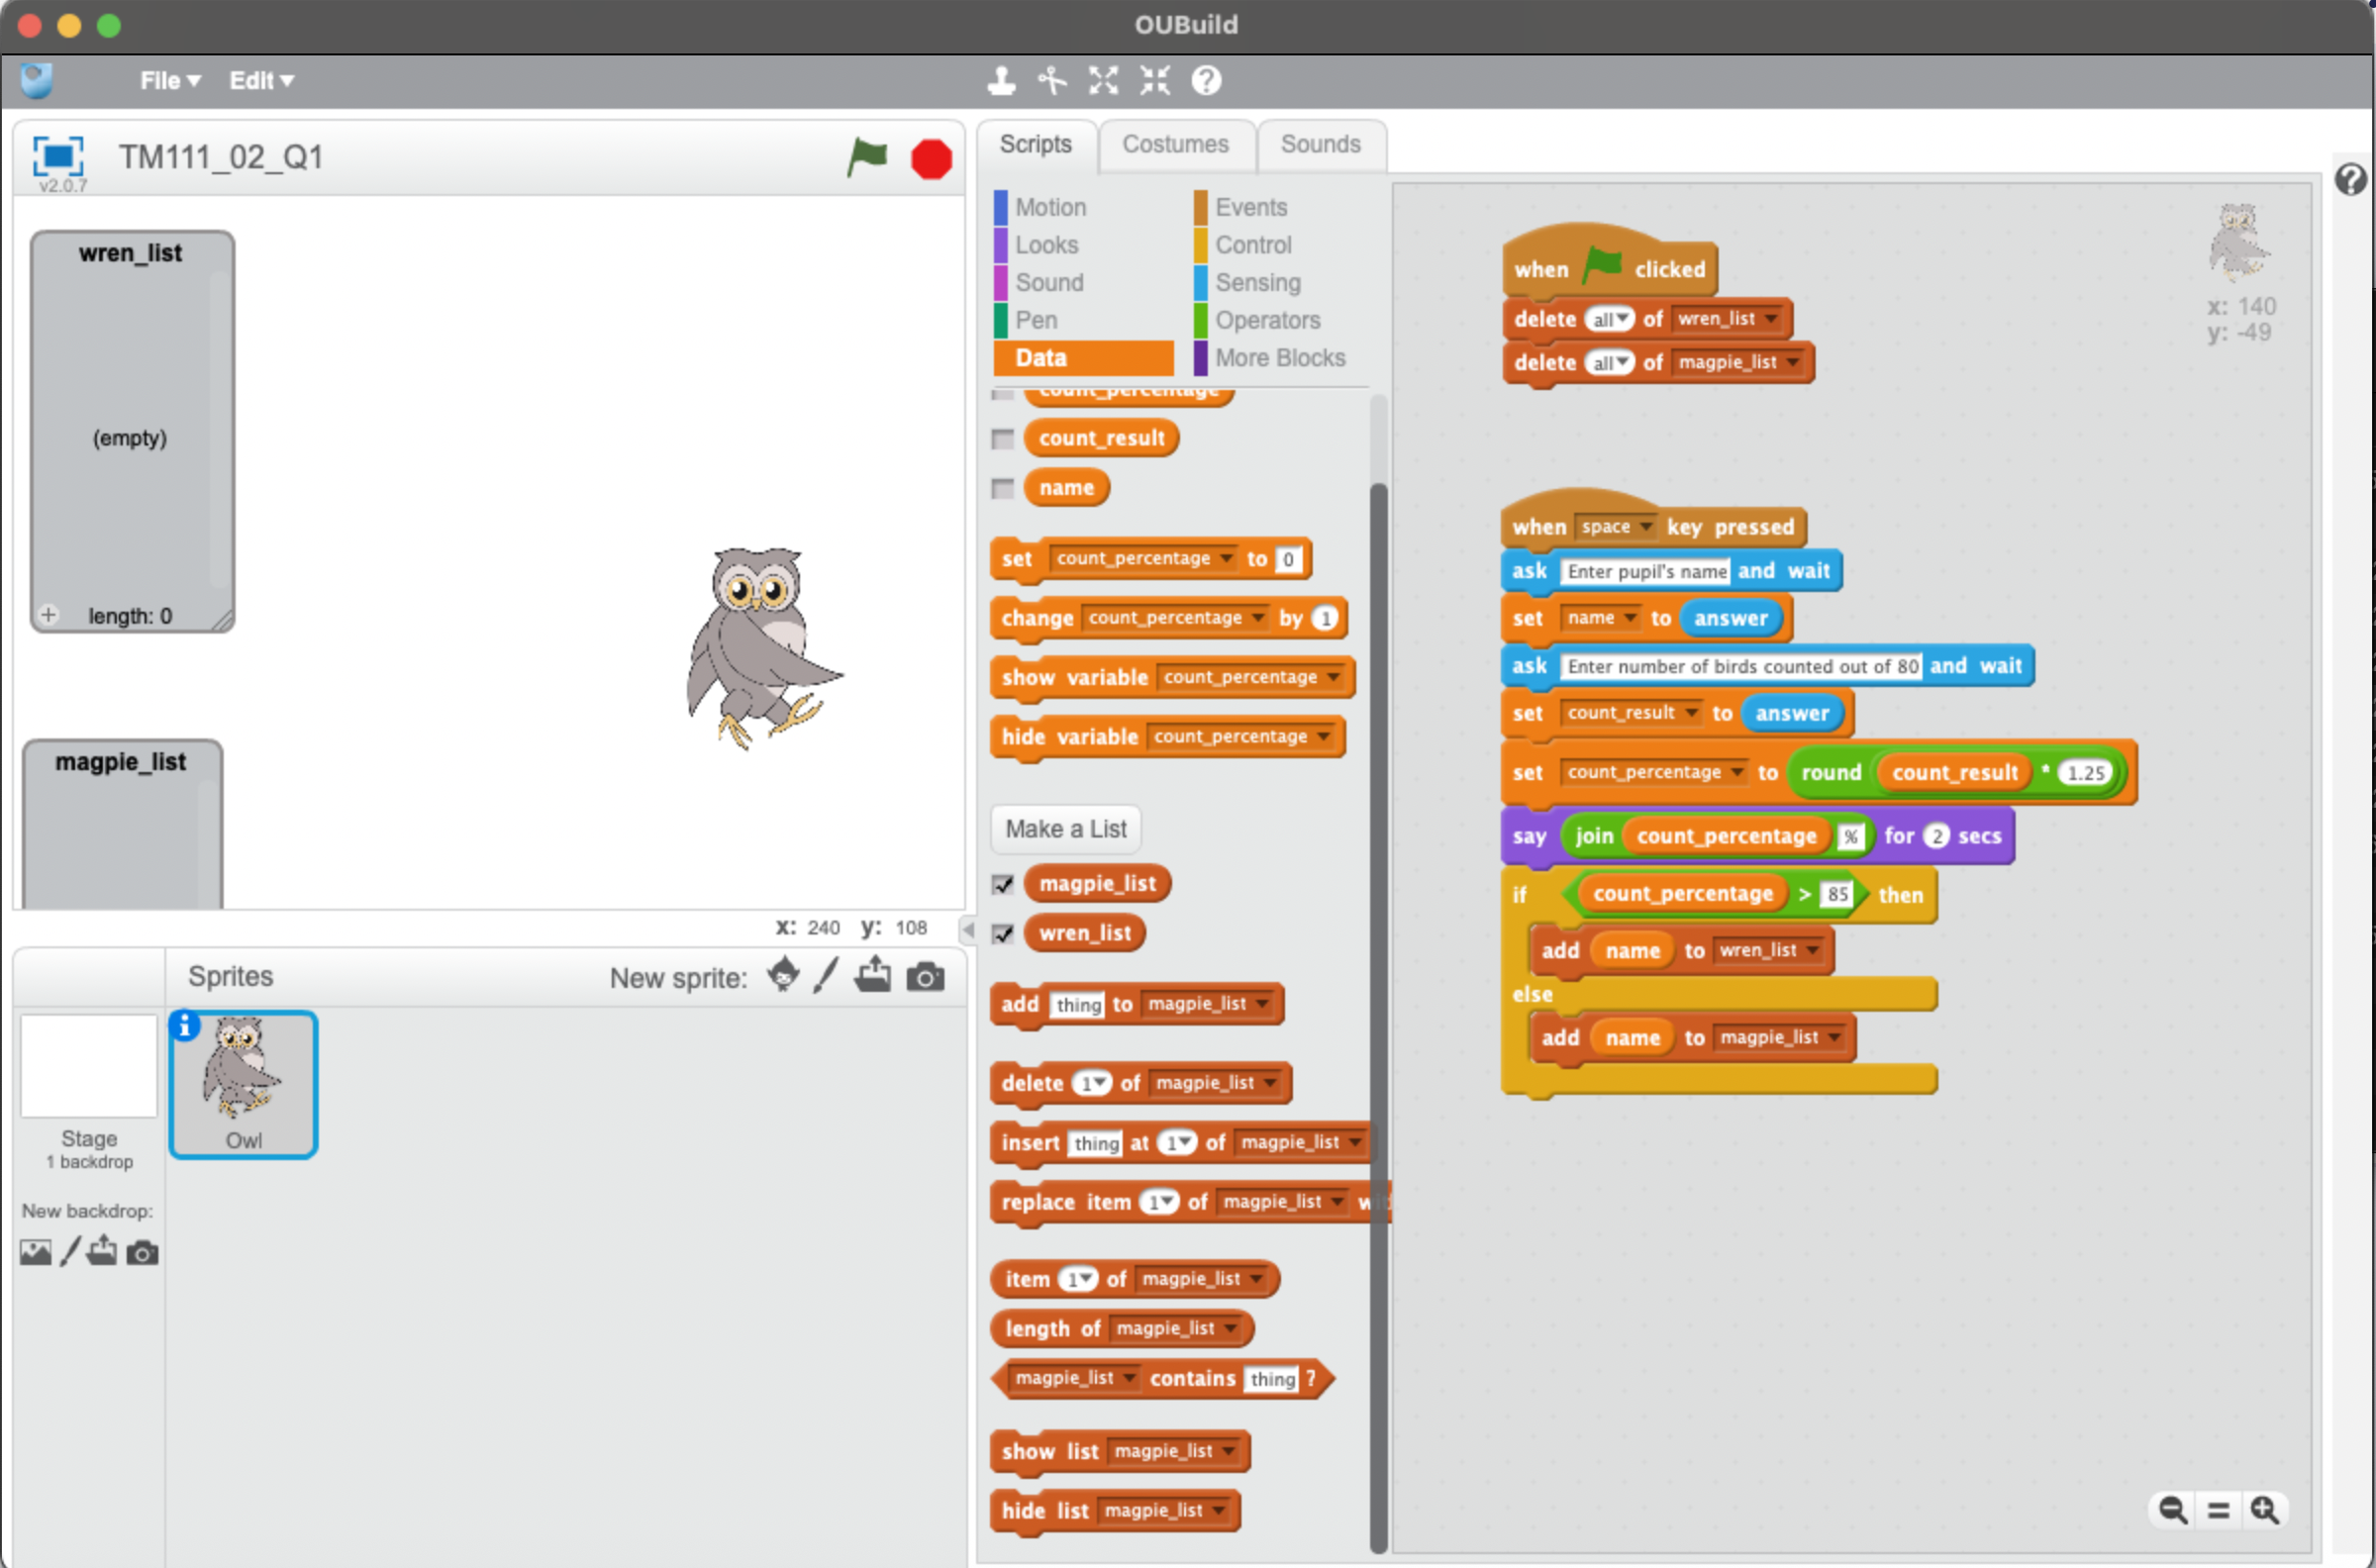
\includegraphics[scale=0.25]{question_1_c.png}

\clearpage

\qpart
\qsubpart

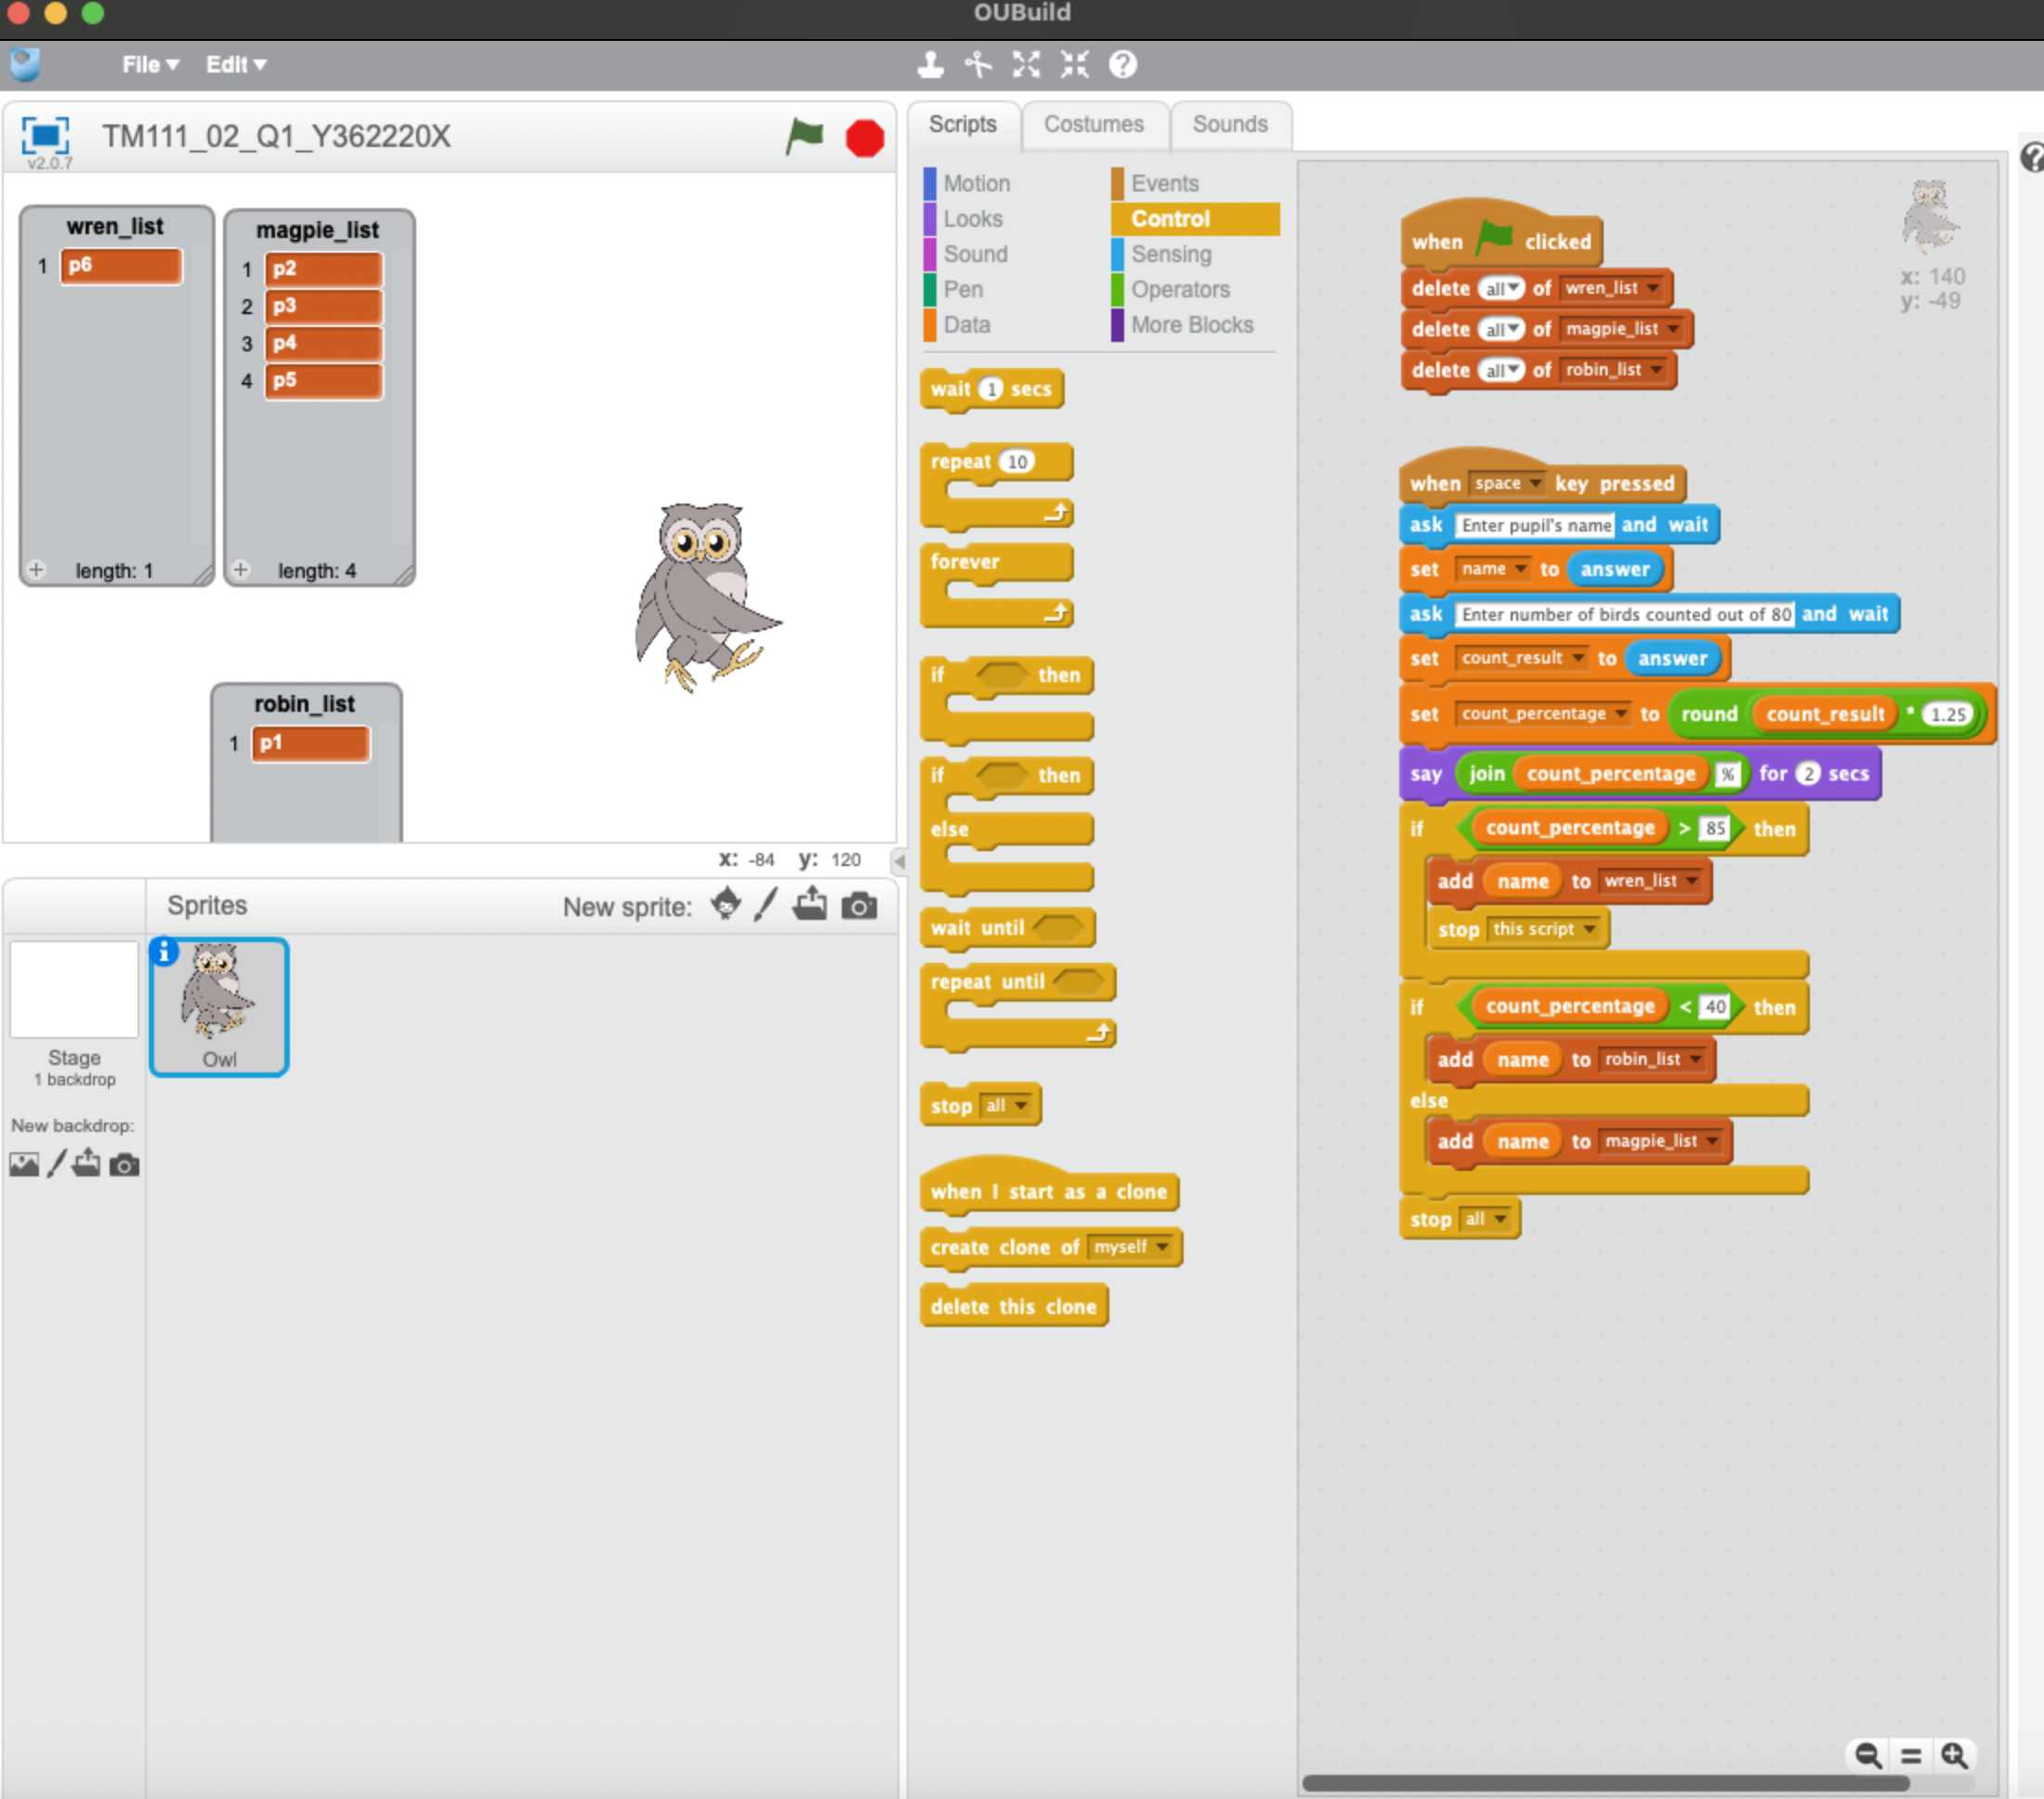
\includegraphics[scale=0.25]{question_1_d.png}

\qsubpart

I could have used three if statements, one for each of the three possible lists.

\end{question}

\begin{question}

  \qpart

  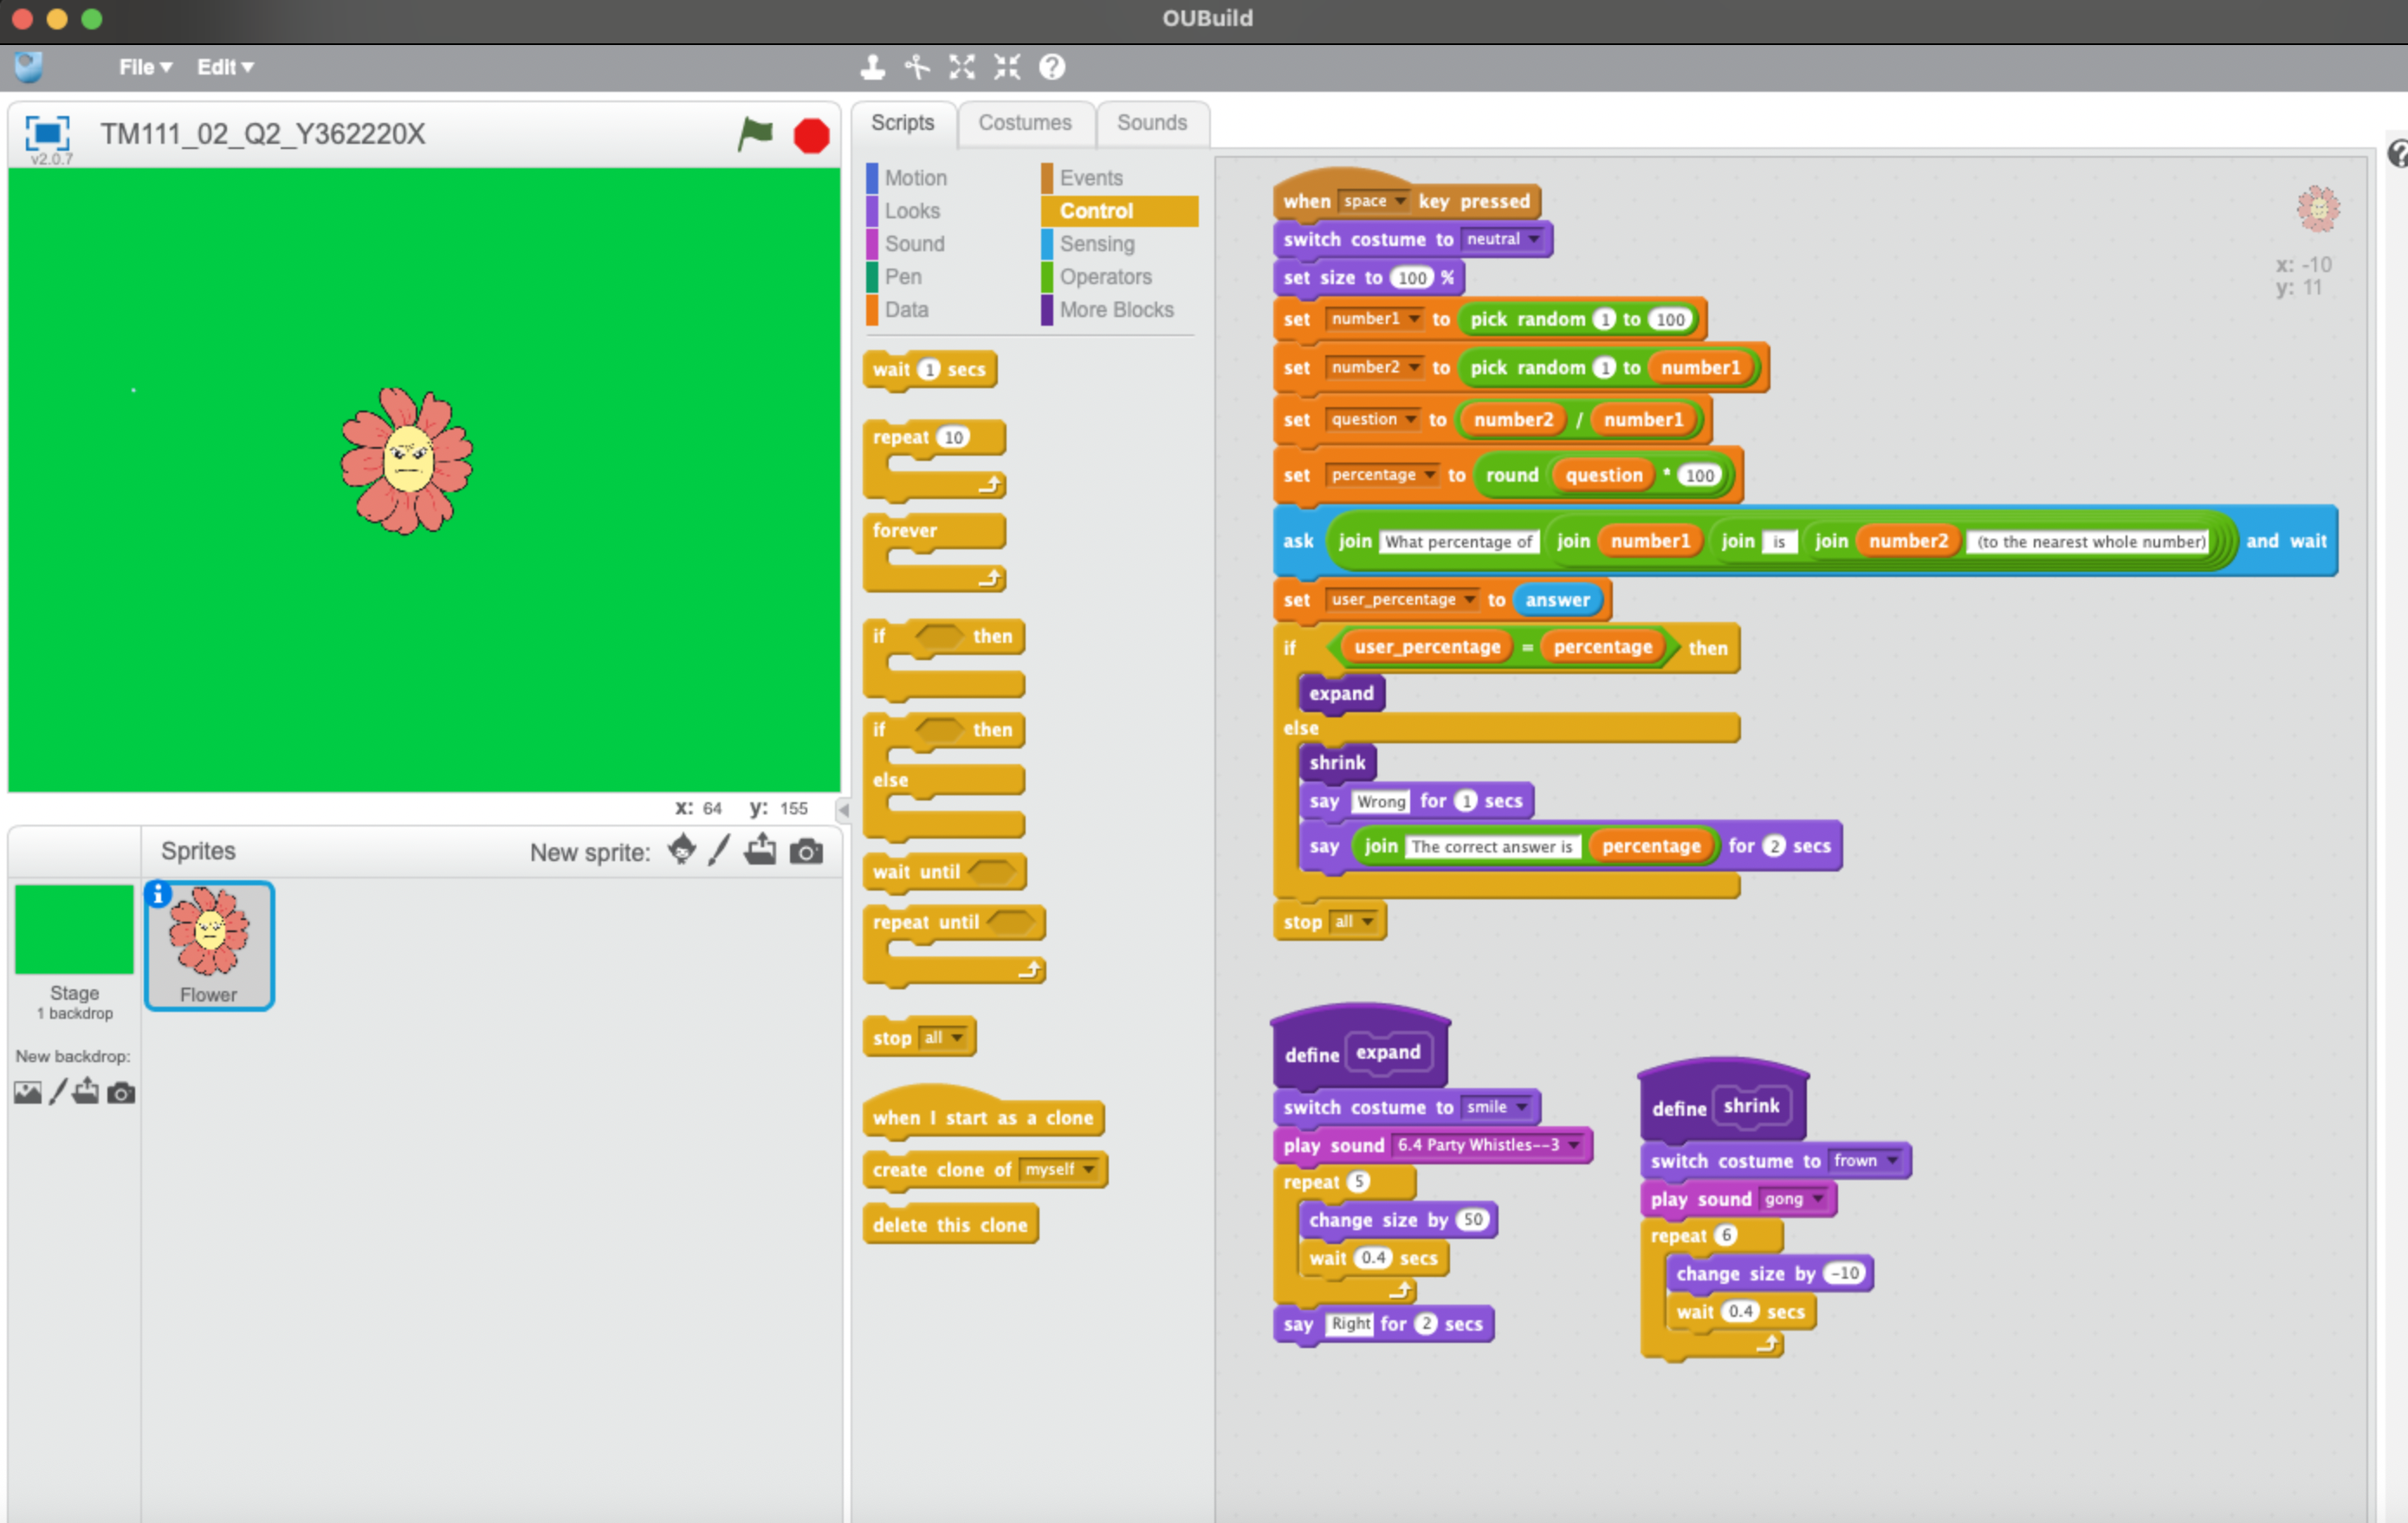
\includegraphics[scale=0.25]{question_2_a.png}

  \qpart


\end{question}

\begin{question}

\qpart

\begin{flushleft}
Clear all variables\par
\quad input word\par
Repeat until end of word\par
if\par
\quad check if character \textit{i} is in the banned list.\par
\quad is on list \textit{i + 1}\par
else\par
\quad add character to \textit{result}\par
say \textit{result}\par
end
\end{flushleft}

\qpart

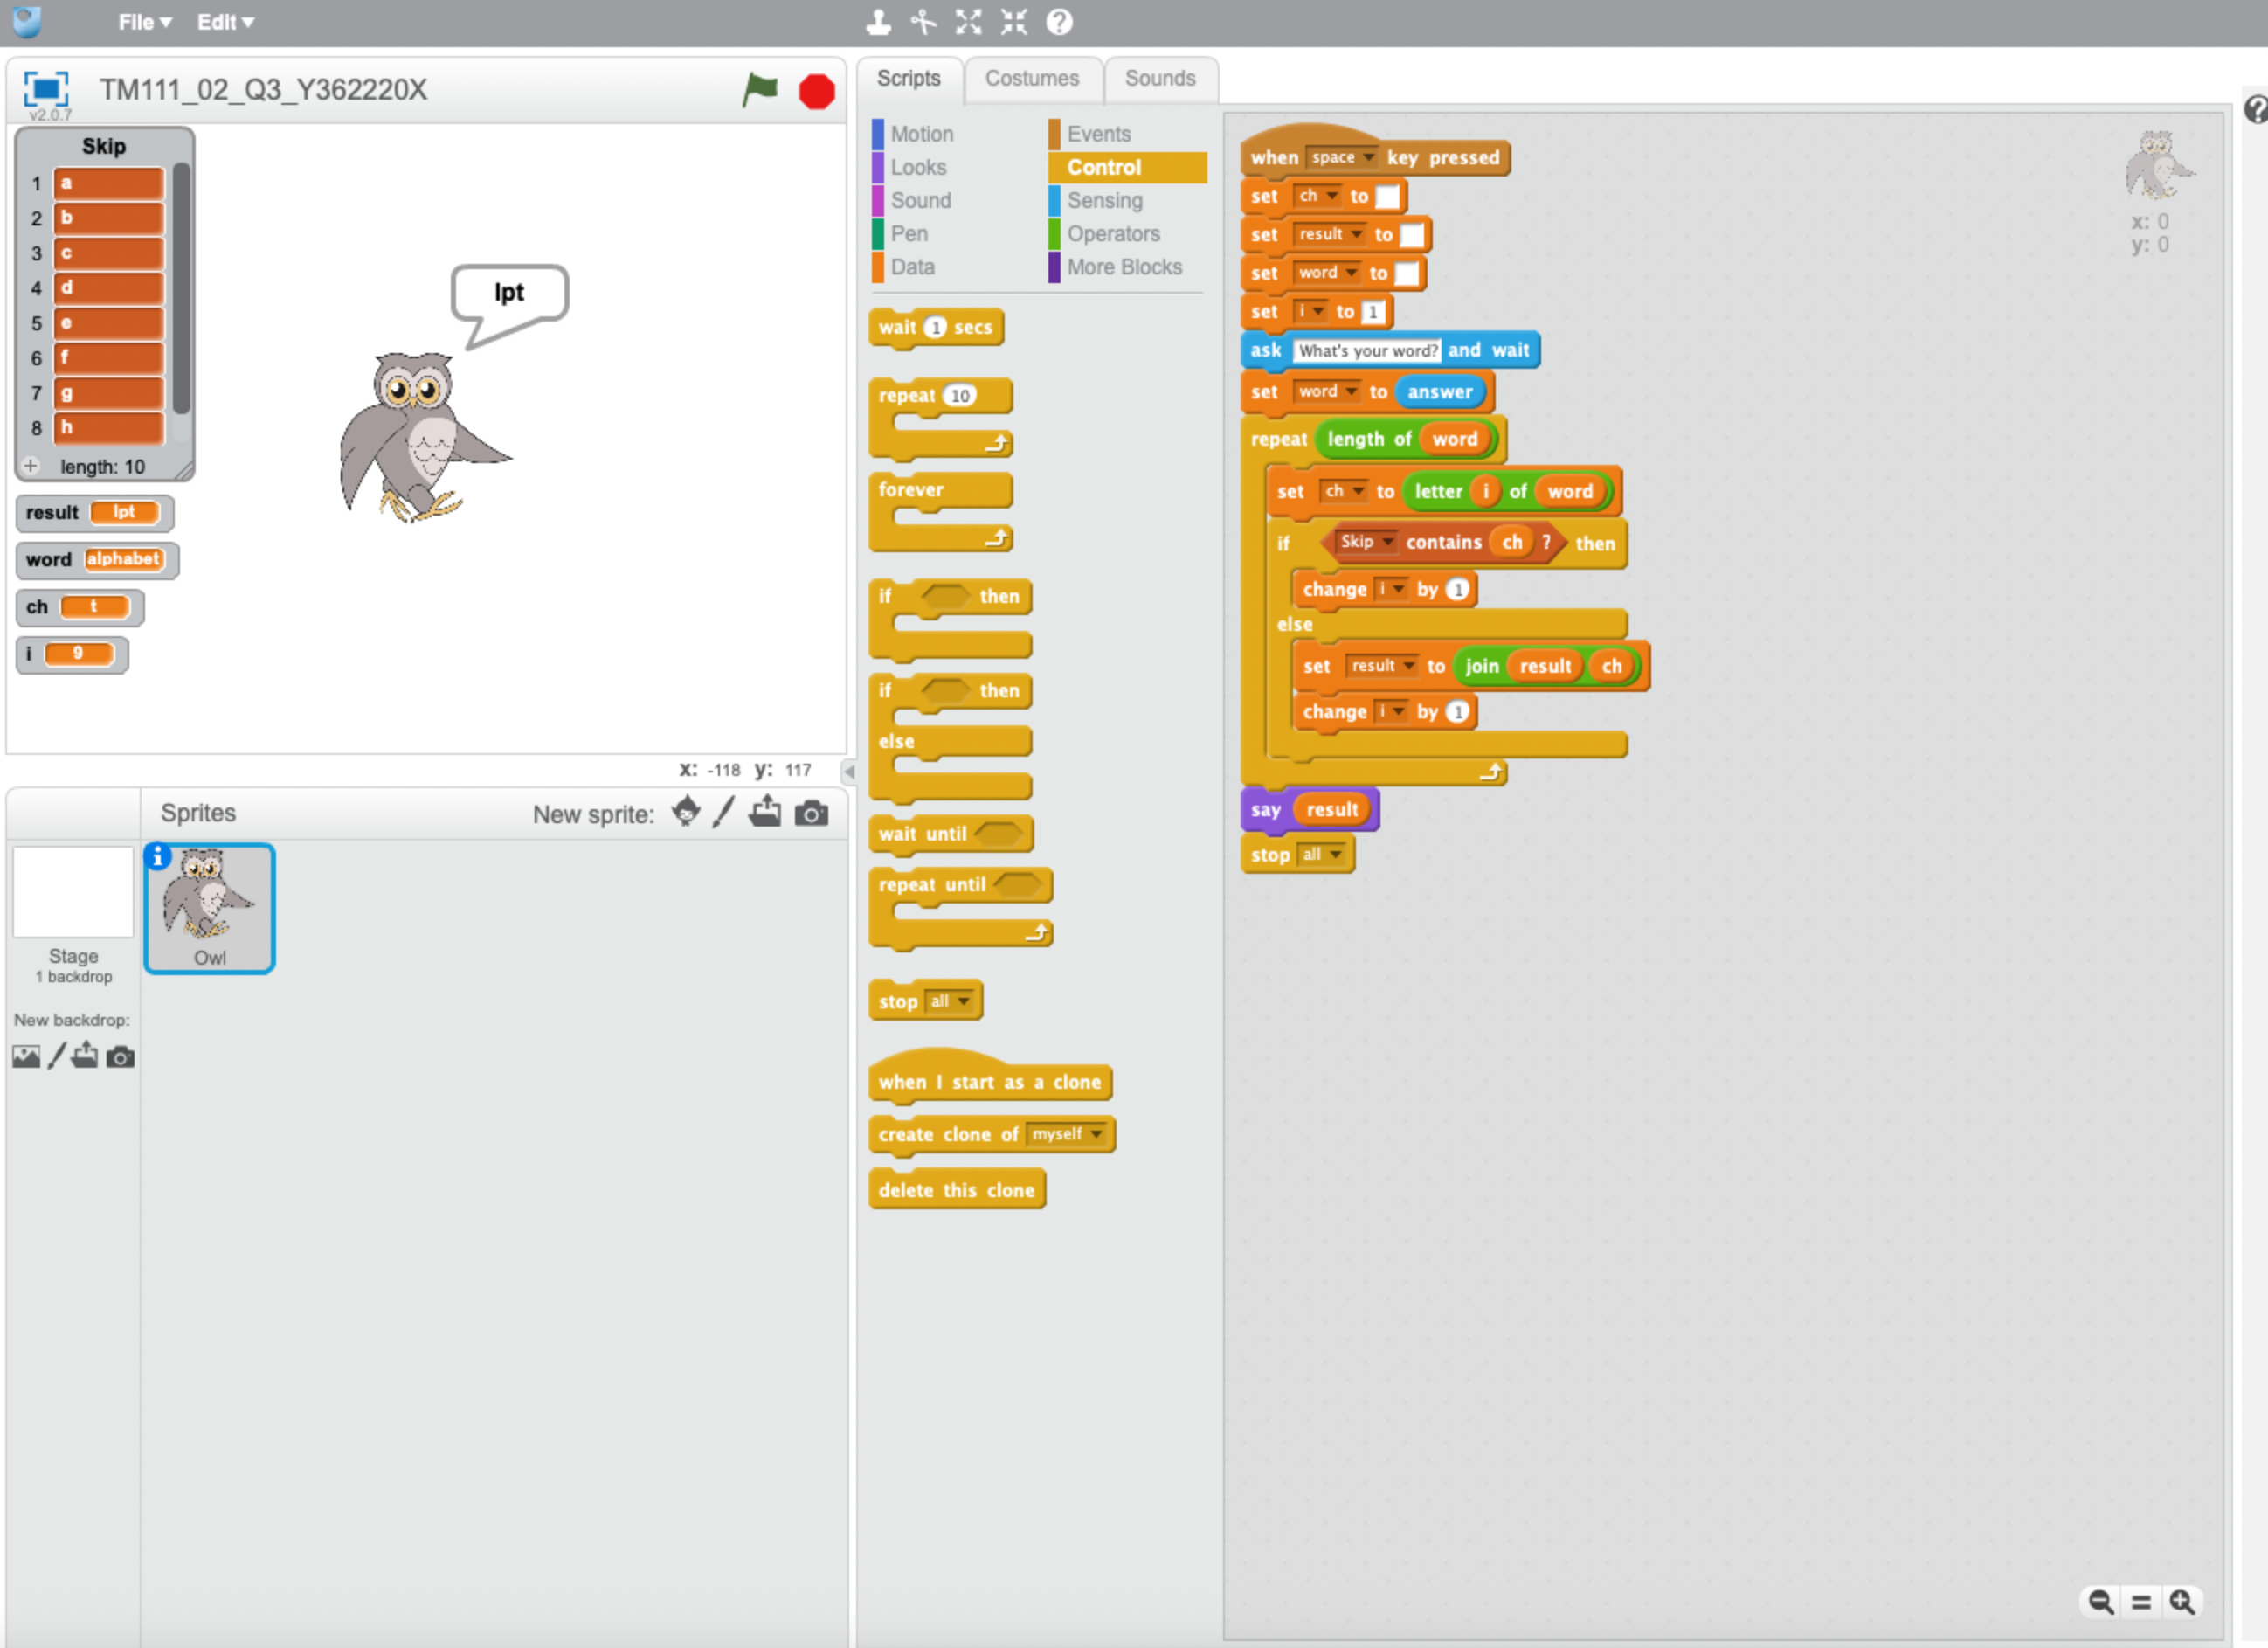
\includegraphics[scale=0.25]{question_3_b.png} 

\qpart

\begin{tabular}{|c|c|c|c|}
    \hline
    Test number & Test purpose & input & Expected result\\
\hline
1 & Frist and last letters are in the first ten letters of the alphabet & apple & ppl\\
\hline
2 & Double letters from the first ten letters of the alphabet & keep & kp\\
\hline
3 & Program works despite case of input & BoOkKeEpEr & oOkKpr\\
\hline
\end{tabular}

\end{question}

\begin{question}

\qpart

\begin{tabular}{|c|c|c|c|c|}
    \hline
    Test number & Test purpose & Existing data & \multicolumn{2}{c|}{Expected result}\\
    \hline
    & & names & least & greatest\\
    \hline
    1 & Least name at position 1, greatest at position 3 & B, I, X, E, R, Q, W, V, D, S & 1 & 3\\
    \hline
    2 & Least name at position 2, greatest at position 1 & Y, A, C, F, H, J, L, M, O, P & 2 & 1\\
    \hline
    3 & Least name at position 1, greatest at position 6 & G, T, K, N, U, Z, H, L, J, O & 1 & 6\\
    \hline
\end{tabular}

\qpart

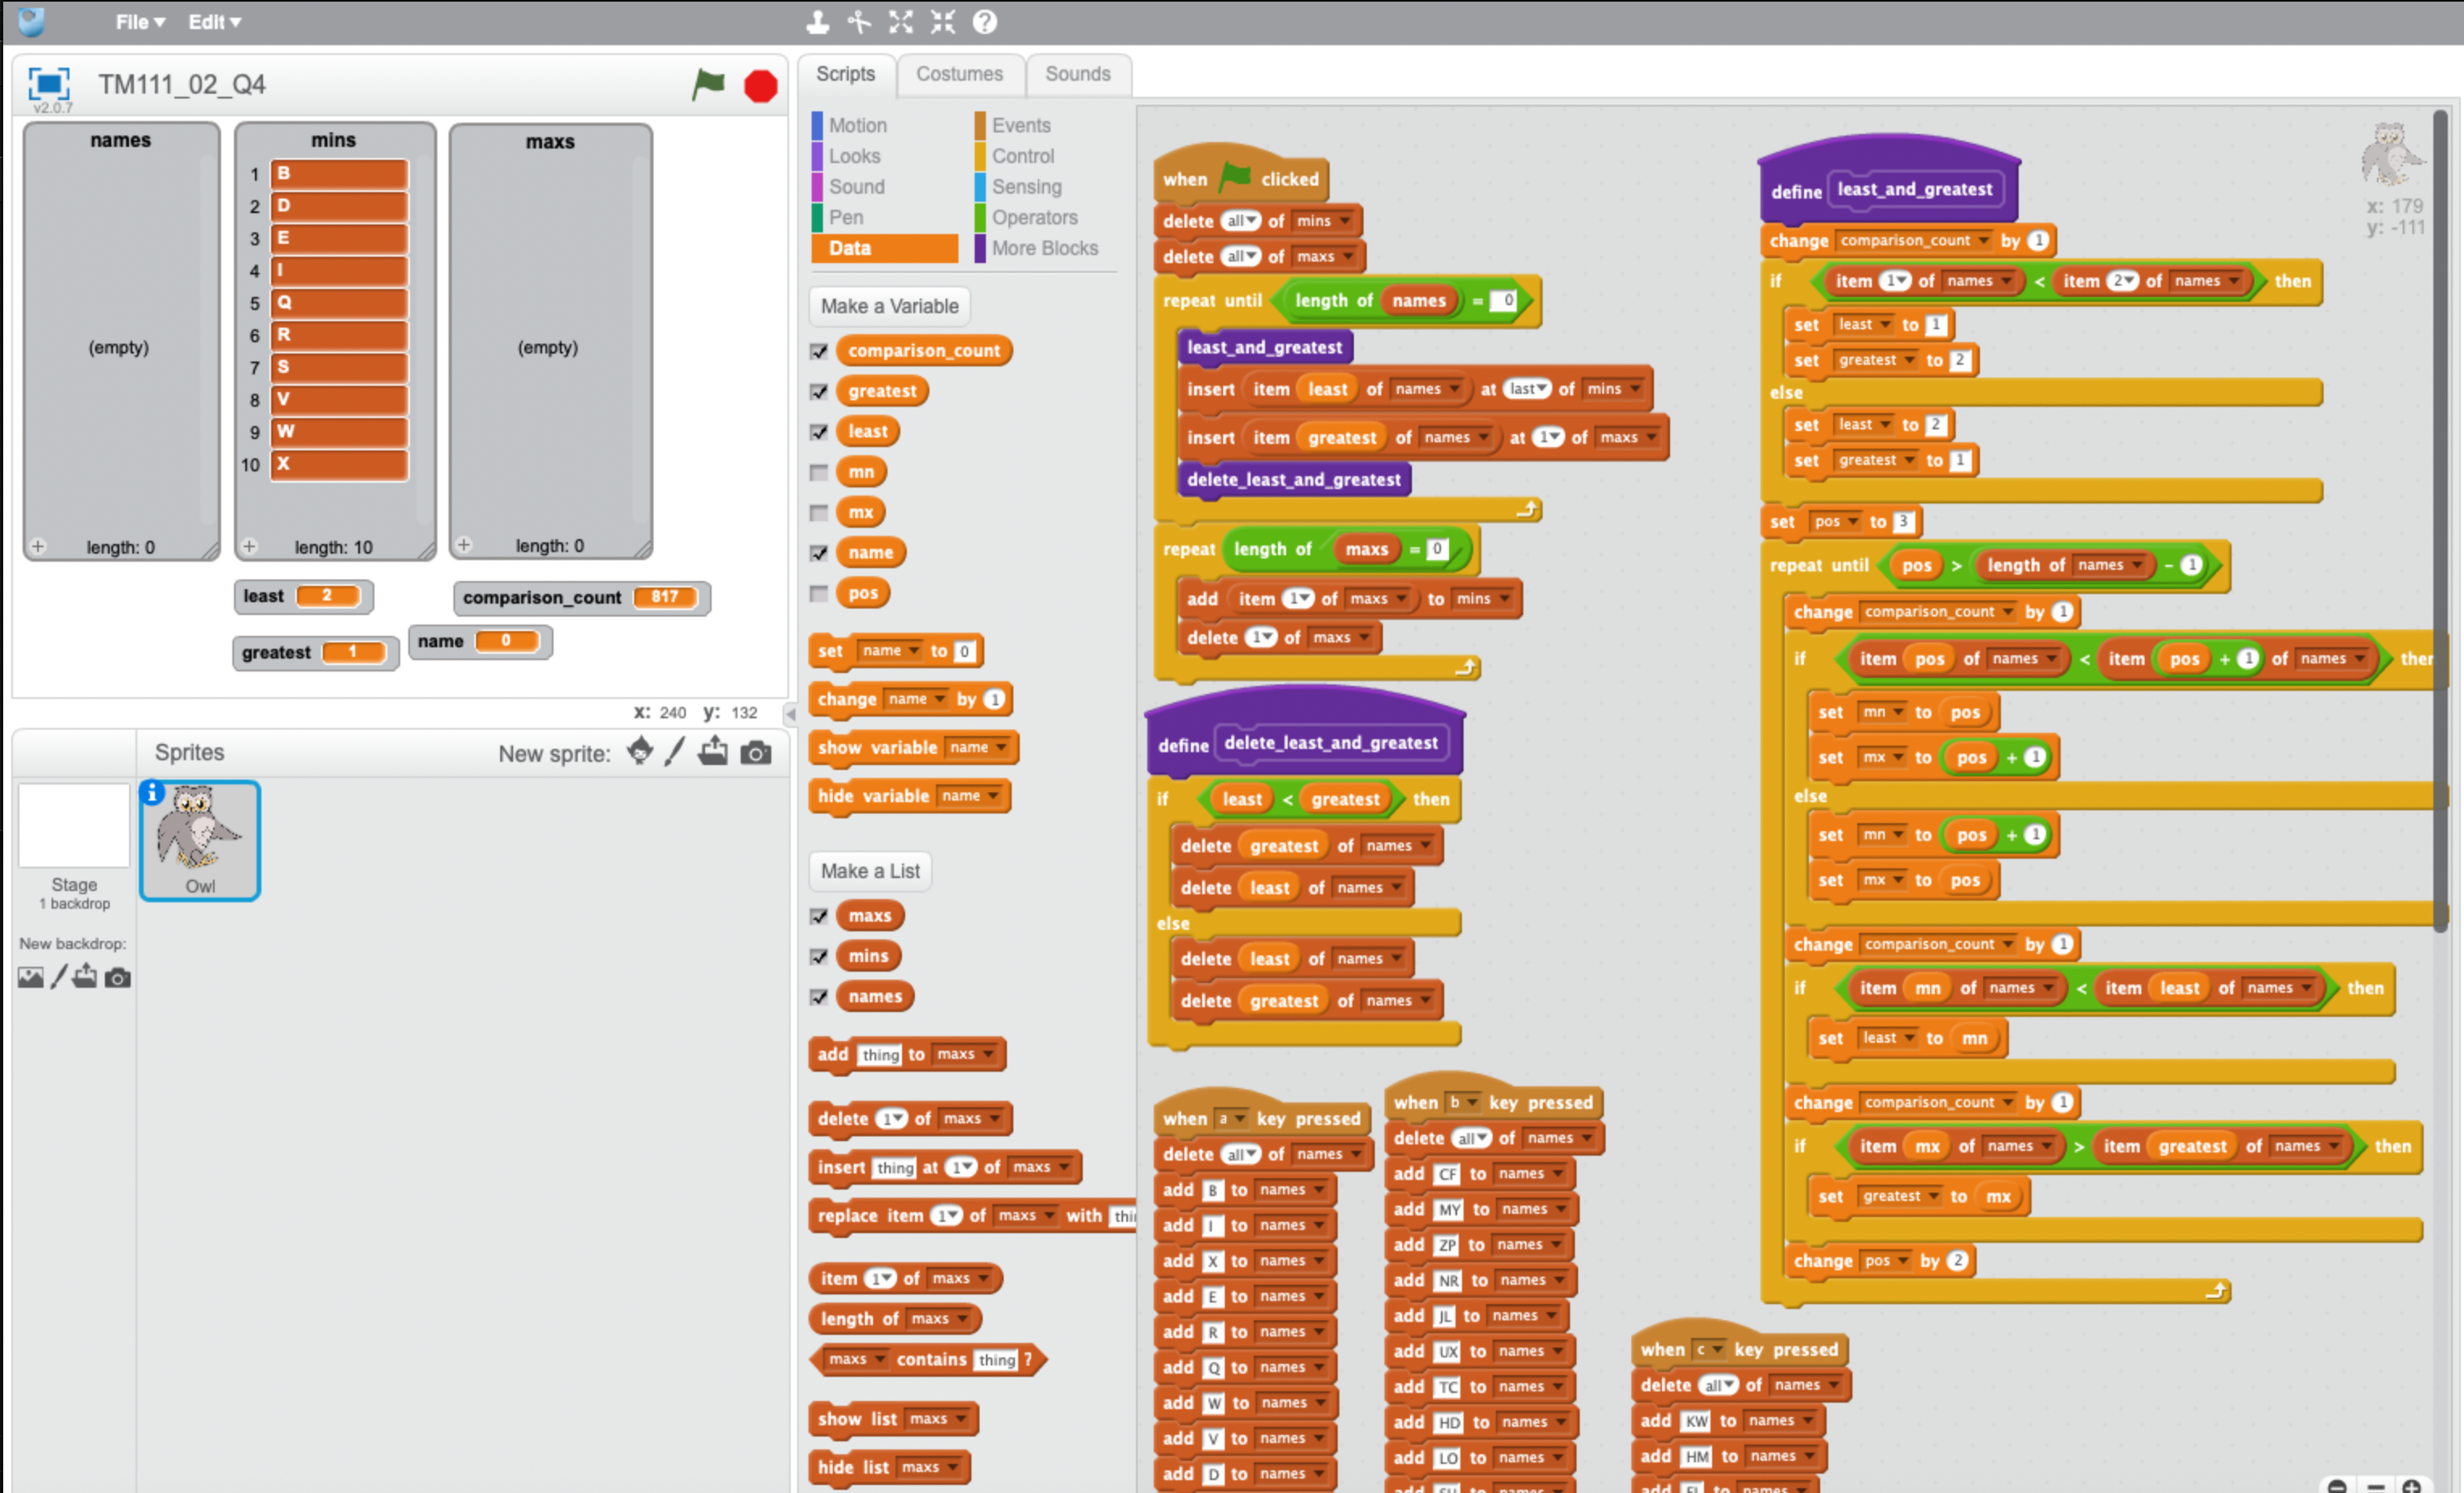
\includegraphics[scale=0.25]{question_4_b.png}

\qpart
\qsubpart

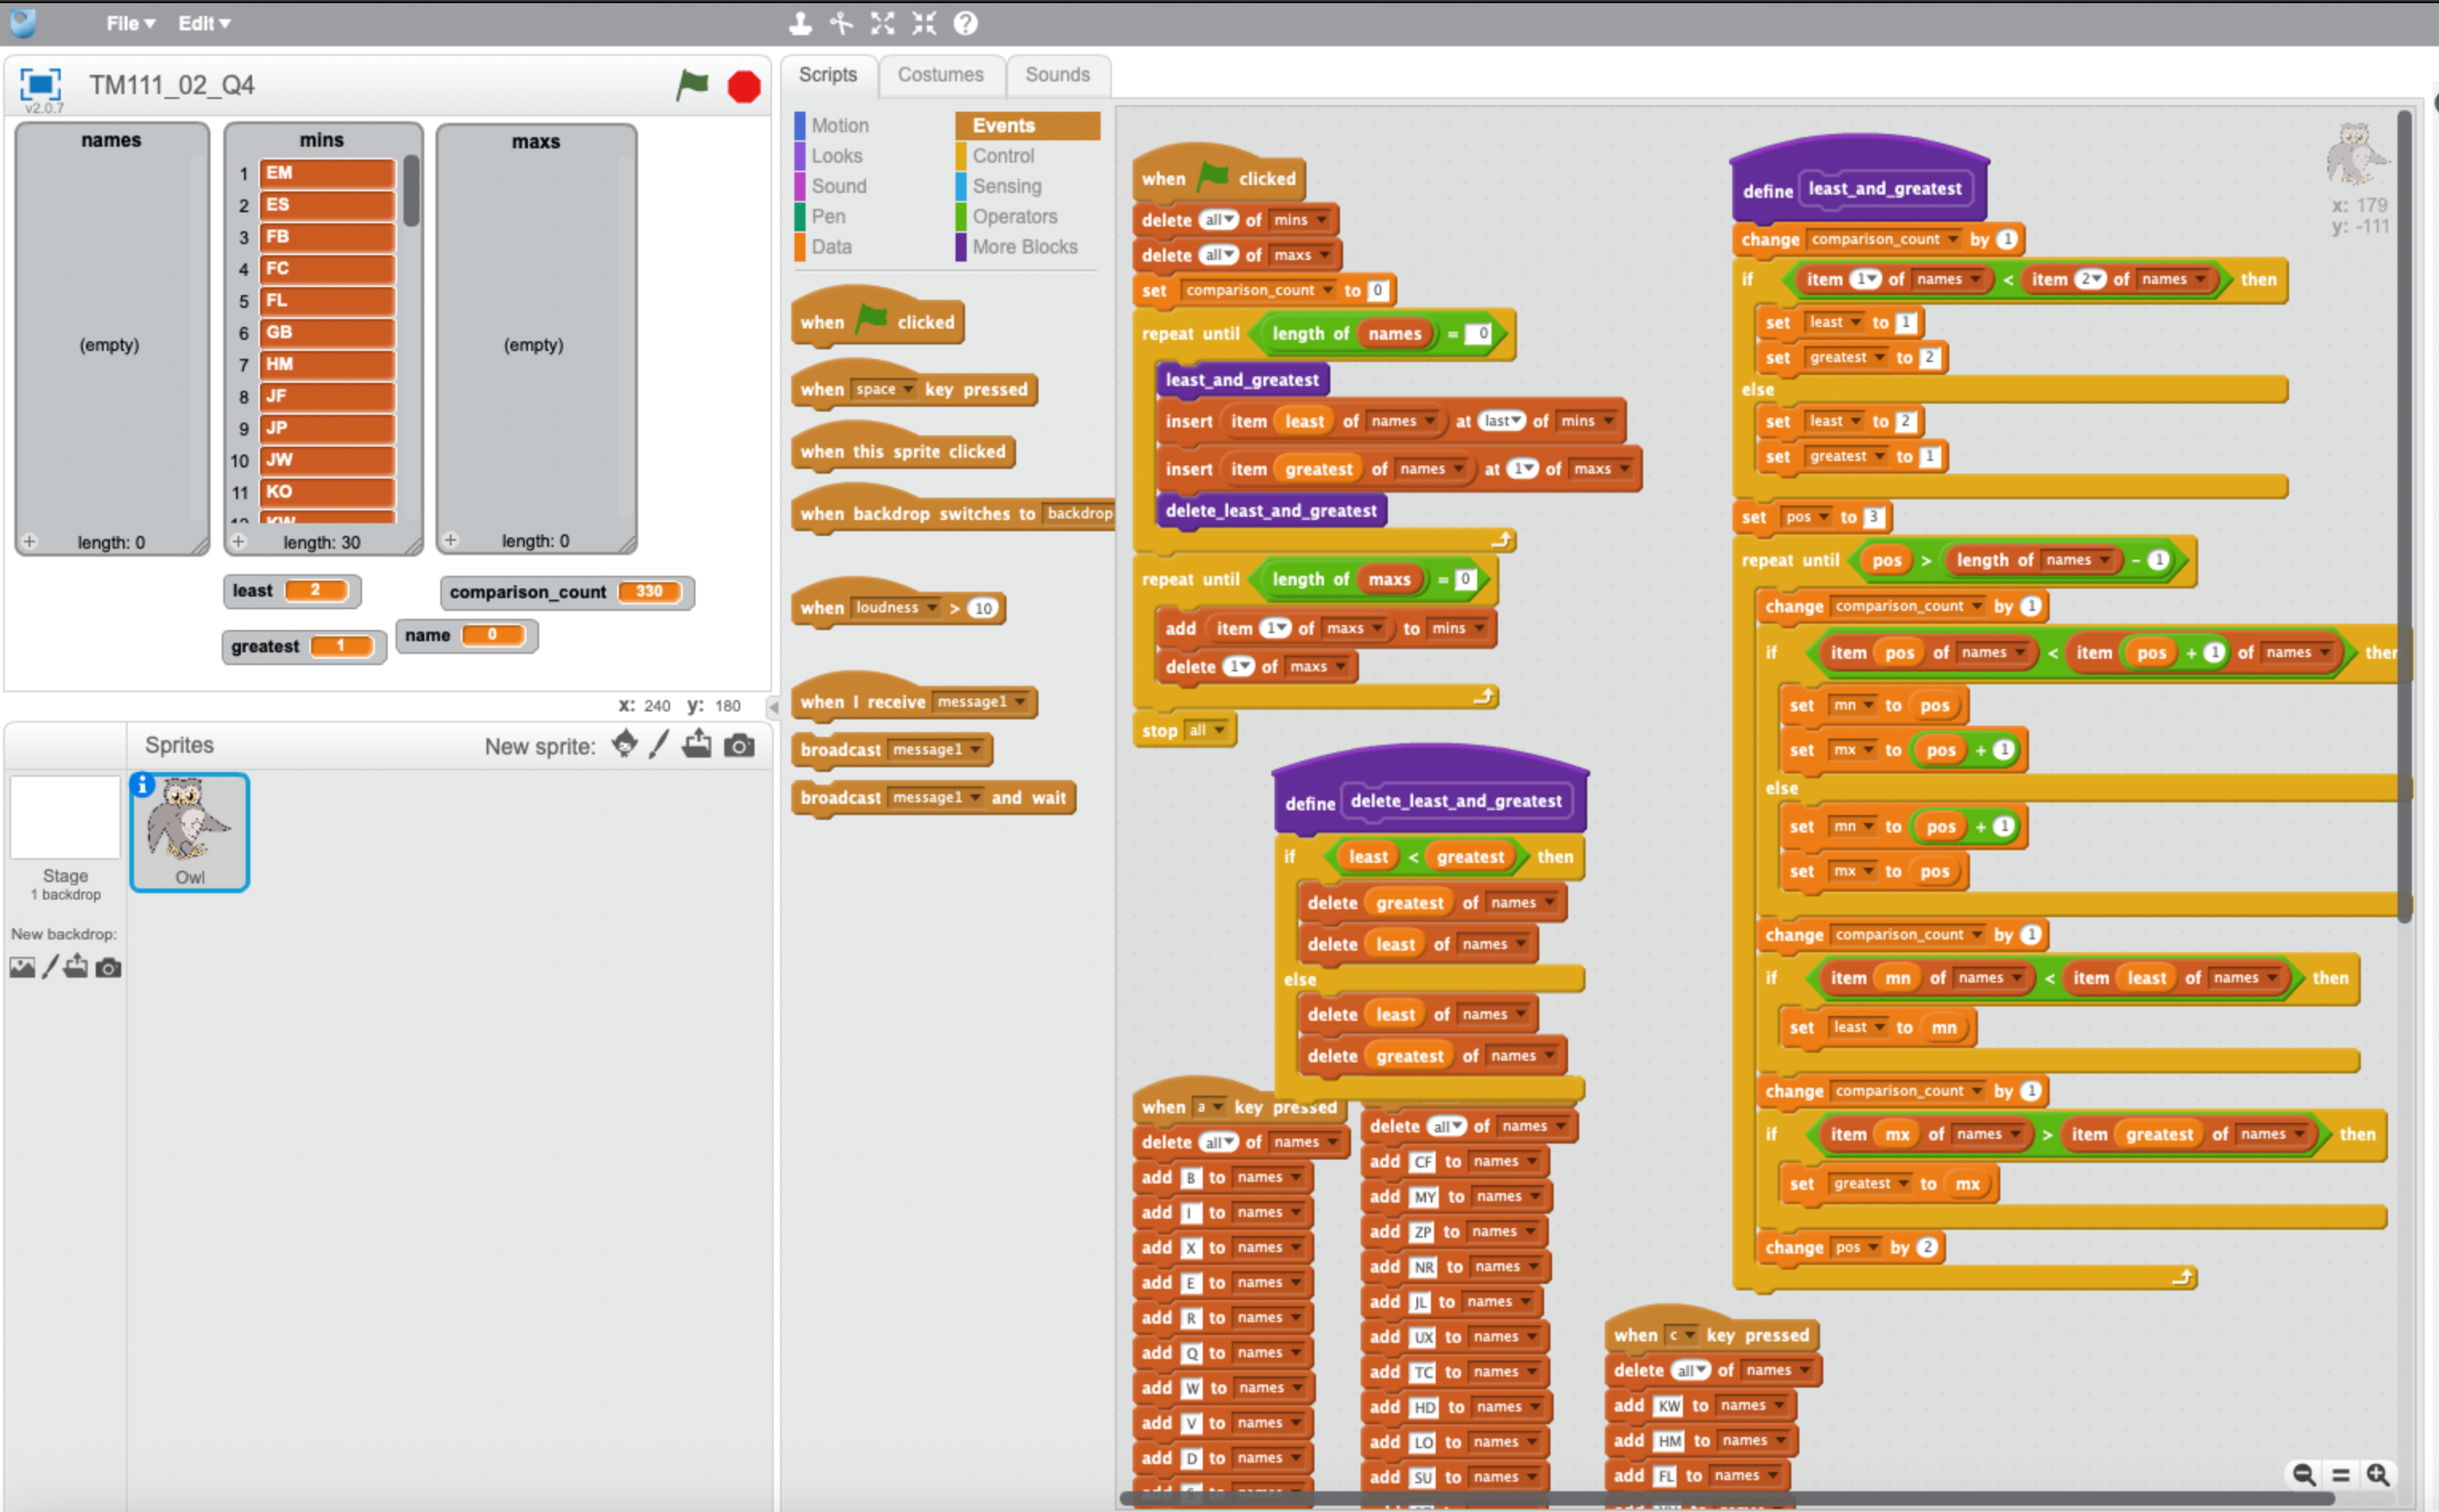
\includegraphics[scale=0.25]{question_4_c.png}

\qsubpart

\begin{tabular}{|c|c|c|c|}
    \hline
    size of list & 10 & 20 & 30\\
    \hline
    Number of comparisons & 35 & 145 & 330  \\
    \hline
\end{tabular}

\qsubpart

The number of comparisons is not linear because the number of comparisons does not increases by
the same amount each time the list increases by the same amount.

\qsubpart

\begin{tabular}{|c|c|c|c|}
    \hline
    size of list (n) & 10 & 20 & 30\\
    \hline
    \(n \times (n-1)\/ 2\) & 45 & 190 & 435  \\
    \hline
    \( 0.75 \times n \times (n-1)\/ 2 \) & 34 & 143 & 327 \\
    \hline
\end{tabular}
 
The number of comparisons  made is close to the theoretical maximum number of comparisons,
which is \(n \times (n-1)\/ 2\), multiplied by 0.75 as program expected a \( 25\% \) improvement.

Given that the number of comparisons has remained close to the theoretical number for our 3 test, we can
assume that this will continue for larger lists. Therefore, if we were sorting a list of \(1000\) names,
the number of comparisons would be approximately \(0.75 \times 1000 \times 999\/ 2 = 374625\).

\qpart

The double selection sort algorithm would lie approximately in the middle of the selection sort and the 
bubble sort 1 algorithm.

\end{question}

\end{document}